\chapter{Komprese dat}
Komprese nebo také komprimace dat je taková transformace dat, která má za cíl úsporu zdrojů při ukládání nebo archivaci a nebo snížení datového toku při přenosu, to vše při současném zachování informace obsažené v datech. Jinými slovy jde o redukci velikosti datových souborů, jehož následkem je úspora paměťových či přenosových kapacit. Postup, při kterém z komprimovaných dat rekonstruujeme data originální, se nazývá dekomprese.

\section{Princip komprese dat}
\label{sekcePrincipKompreseDat}
Data velmi často obsahují tzv. redundantní\footnote{Redundance znamená informační nadbytek, např. vícenásobný výskyt slov v textu.} informaci, toho právě využívá komprese -- data jsou zpracována tak, aby byla redundance minimalizována. Jak lze vidět na obrázku \ref{kompreseDekomprese}, je na vstupní data použita operace komprese. Operací dekomprese dostaneme poté data rekonstruovaná -- v závislosti na použité kompresní metodě, respektive na požadavcích získáme buď data přesně odpovídající původním a nebo pouze částečná. Z tohoto hlediska rozlišujeme dva typy kompresních metod: ztrátové a bezeztrátové.

\begin{figure}[!htb]
\centering
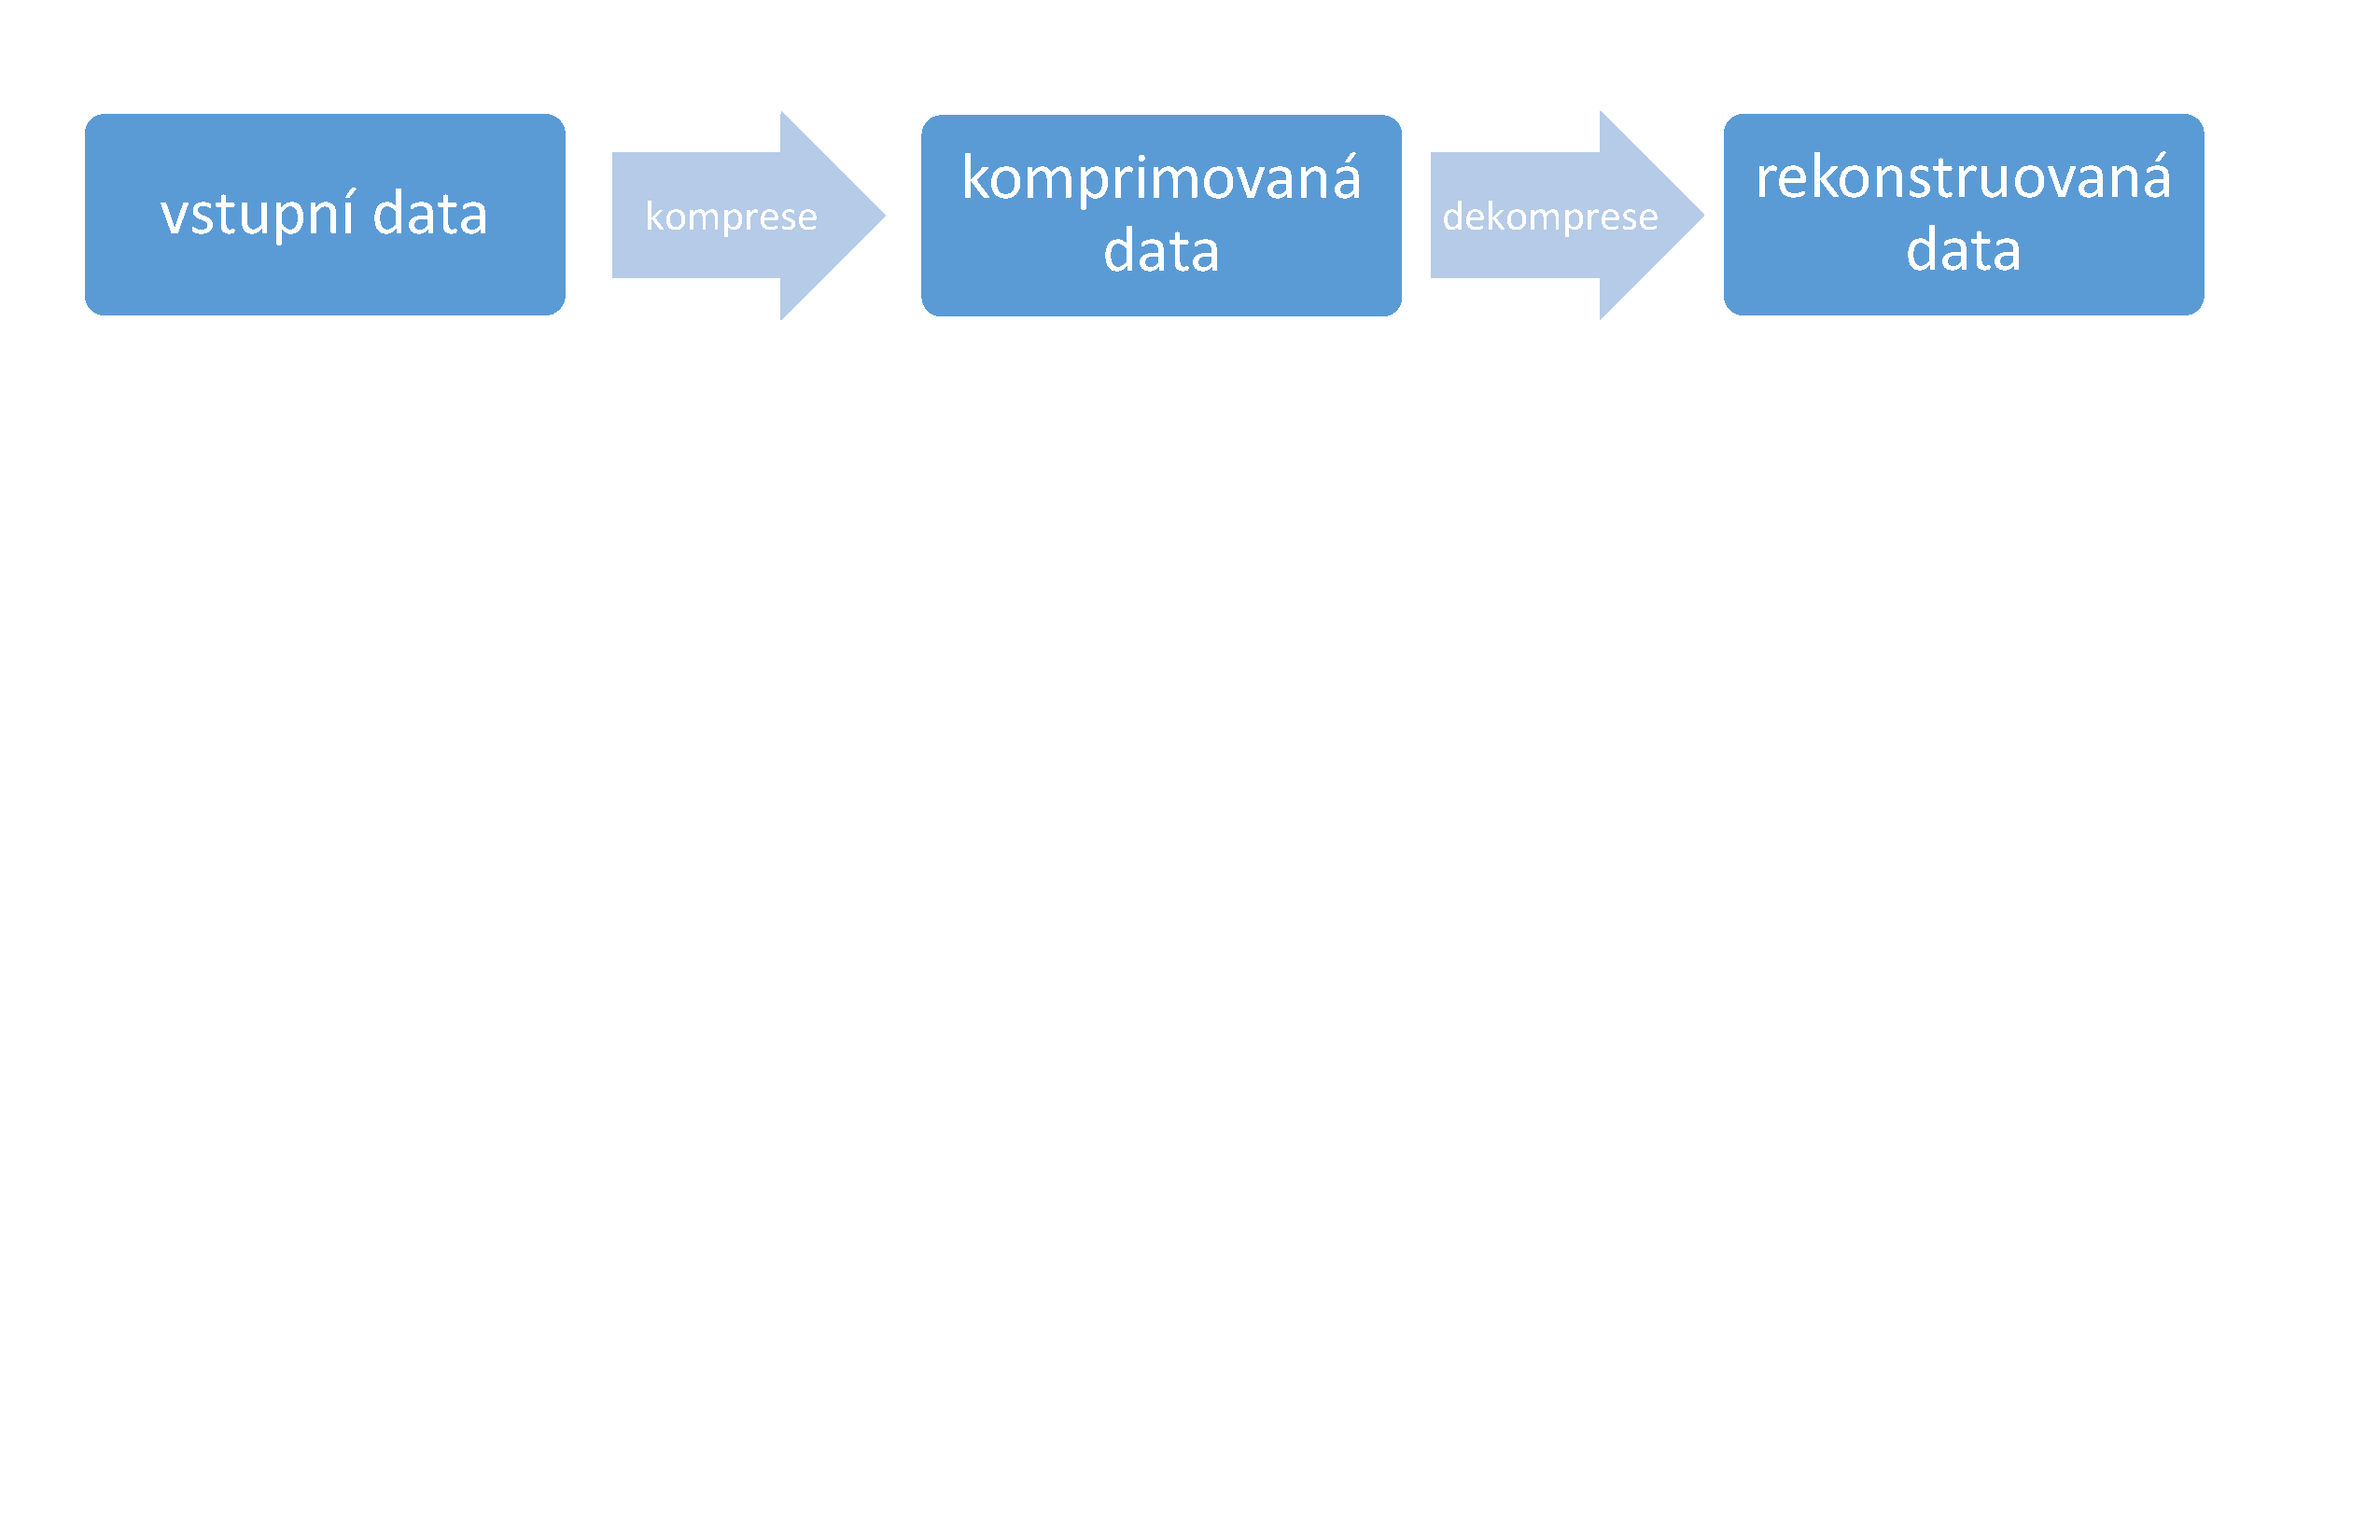
\includegraphics[trim=0 610 60 55, clip, angle=0, width=150mm]{kompreseDekomprese}
\caption{Princip komprese}
\label{kompreseDekomprese}
\end{figure}


\section{Typy kompresních metod}
Jak název napovídá, při ztrátové kompresi ztratíme část informace obsaženou v původních datech, respektive jsou původní data pouze aproximována.  Toto nám nemusí vadit například u obrázků, zvuku a videí, kde je využito nedokonalosti lidských smyslů. Lidské ucho nedokáže například slyšet velmi vysoké frekvence. Má smysl v datech určených k poslechu zachovávat informaci, kterou nemůže člověk slyšet? Častá odpověď je \uv{ne}. Tohoto principu využívá mnoho kompresních metod, například známý zvukový formát MP3. Odstraněním \uv{nepotřebné} informace z dat je dosaženo ještě větší redukce objemu. 

Naopak v případě bezeztrátových metod je při kompresi zachována veškerá informace a při dekompresi
jsou rekonstruována původní data. Těchto metod se využívá převážně tam, kde není možné původní data jakkoliv pozměnit. Například data ve formátech XML a JSON, kterým se věnuji v této práci, si nemůžeme dovolit pozměnit (přestanou mít původní význam), nebo dokonce ztratit.

\section{Charakteristika komprese}
Kompresní algoritmy lze hodnotit z mnoha různých úhlů pohledu. Můžeme měřit složitost algoritmu, rychlost, jakou data komprimována a dekomprimována (to může být ovlivněno výkonem stroje, na kterém algoritmus běží), jak moc odpovídají rekonstruovaná data původním atd.
Jednou z nejčastějších charakteristik je, logicky ze smyslu komprese vy\-plý\-va\-jí\-cí, tzv. kompresní poměr, který vyjadřuje velikost komprimovaných dat vůči původním, lze ho zapsat následujícím  vztahem:
\begin{equation}
\texttt{kompresní poměr} = \frac{\texttt{délka původních dat}}{\texttt{délka komprimovaných dat}}.
\end{equation}

Další sledovanou charakteristikou je tzv. úspora místa, která je vyjádřena jako:
\begin{equation}
\texttt{úspora místa} = \texttt{1 - kompresní poměr$^{-1}$}.
\end{equation}

Mějme například 2D obrázek o velikosti $256\times256$ pixelů, který zabírá 65536 bytů. Obrázek zkomprimujeme a zabírá-li komprimovaná verze 16384 bytů, můžeme říct, že kompresní poměr je $4:1$ a úspora místa 75 \%. 

\section{Míra informace v datech}
